\documentclass[11pt,a4paper]{article}

\usepackage[a4paper,left=2.2cm,right=2.2cm,top=2.1cm,bottom=2.3cm]{geometry}
\usepackage{fontspec}
\usepackage[table]{xcolor}
\usepackage{graphicx}
\usepackage{booktabs}
\usepackage{array}
\usepackage{tabularx}
\usepackage{titlesec}
\usepackage{caption}
\usepackage{enumitem}
\usepackage{float}
\usepackage{fancyhdr}
\usepackage{microtype}
\usepackage[hidelinks]{hyperref}

\setmainfont{Charter}[BoldFont={Charter Bold},ItalicFont={Charter Italic},BoldItalicFont={Charter Bold Italic}]
\newfontfamily\headfont{Avenir Next}[Ligatures=TeX,UprightFont={* Medium},BoldFont={* Demi Bold},ItalicFont={* Medium Italic}]
\newfontfamily\headfontreg{Avenir Next}[Ligatures=TeX,UprightFont={* Regular}]
\setmonofont{Menlo}[Scale=0.8]

\definecolor{ink}{HTML}{1E1C1A}
\definecolor{oxblood}{HTML}{7A2E2E}
\definecolor{ochre}{HTML}{B5832A}
\definecolor{olive}{HTML}{5F6B3A}
\definecolor{warmgrey}{HTML}{8A837A}
\definecolor{paper}{HTML}{F3EFE7}
\definecolor{ourrow}{HTML}{F5ECE9}
\color{ink}

\hypersetup{colorlinks=true,linkcolor=oxblood,citecolor=oxblood,urlcolor=oxblood,
  pdftitle={SpinTrace: tracing paraphrased news to its source},pdfauthor={CSD358 team}}

\linespread{1.03}
\setlength{\parindent}{0pt}
\setlength{\parskip}{0.4em}
\frenchspacing

\titleformat{\section}{\headfont\bfseries\large\color{ink}}{\thesection}{0.7em}{}[\vspace{0.1em}{\color{oxblood}\titlerule[0.5pt]}]
\titlespacing*{\section}{0pt}{1.1em}{0.5em}
\titleformat{\subsection}{\headfont\bfseries\normalsize\color{ink}}{\thesubsection}{0.6em}{}
\titlespacing*{\subsection}{0pt}{0.9em}{0.15em}
\titleformat{\paragraph}[runin]{\headfont\bfseries\small\color{ink}}{}{0pt}{}[.]
\titlespacing*{\paragraph}{0pt}{0.5em}{0.6em}

\captionsetup{font={small},labelfont={color=oxblood},textfont={},labelsep=period,skip=5pt,
  justification=raggedright,singlelinecheck=false}
\DeclareCaptionFont{avenir}{\headfontreg}
\captionsetup{font={avenir,small}}
\setlength{\textfloatsep}{12pt plus 2pt minus 2pt}
\setlength{\floatsep}{10pt plus 2pt minus 2pt}

\setlist{itemsep=0.15em,topsep=0.2em,parsep=0pt,leftmargin=1.4em}

\pagestyle{fancy}
\fancyhf{}
\renewcommand{\headrulewidth}{0pt}
\fancyfoot[C]{\headfontreg\footnotesize\color{warmgrey}\thepage}

% tables: Avenir header on a paper tint, hairline rules, our method's row tinted
\setlength{\aboverulesep}{0.25ex}
\setlength{\belowrulesep}{0.35ex}
\setlength{\heavyrulewidth}{0.6pt}
\setlength{\lightrulewidth}{0.35pt}
\arrayrulecolor{warmgrey}
\newcommand{\hd}[1]{{\headfont\bfseries\footnotesize #1}}
\newcommand{\hrow}{\rowcolor{paper}}
\newcommand{\ours}{\rowcolor{ourrow}}
\newcommand{\code}[1]{\texttt{#1}}
\newcolumntype{R}{>{\raggedleft\arraybackslash}X}
\newcolumntype{P}[1]{>{\raggedright\arraybackslash}p{#1}}
\newcolumntype{L}{>{\raggedright\arraybackslash}X}
\newenvironment{wdlist}{\begin{minipage}[t]{\linewidth}\raggedright\vspace{1pt}\begin{itemize}[leftmargin=1.1em,label=\textbullet,itemsep=3.5pt,topsep=0pt,parsep=0pt,partopsep=0pt]}{\end{itemize}\vspace{5pt}\end{minipage}}
\newcommand{\hdd}[2]{\hd{\begin{tabular}[b]{@{}r@{}}#1\\#2\end{tabular}}}

\begin{document}

{\headfont\bfseries\LARGE SpinTrace\par}
\vspace{0.25em}
{\headfont\large Tracing paraphrased news to its source with a polite crawler\par}
\vspace{0.7em}
{\headfontreg\small Nishita Kadali\quad\textcolor{warmgrey}{/}\quad Pustak Pathak\par
CSD358 Information Retrieval, mid-term hackathon, Track 4: web crawling, freshness and web integrity\par
October 2026\par}
\vspace{0.4em}

\section{Problem and track relevance}

In August 2023 NewsGuard gave 43 AI-rewritten articles from content farms to Grammarly's premium plagiarism checker. It could not identify the original source of 34 of them, a 79\% failure rate~\cite{ng2023}. The farms take a story from a mainstream outlet, have a language model reword it, and publish the result as their own. NewsGuard's tracking page now counts 3,749 AI content-farm sites~\cite{ng2026}. The checker fails for a structural reason: it looks for text pulled verbatim, and a paraphrase has very little of it.

A web crawler has the same blind spot. Its ``content seen?'' check fingerprints each page and compares sets of word shingles, which catches mirrors and light edits~\cite{broder1997,manku2007,iir2008}. A paraphrase shares almost no word 5-grams with its source; in our tests MinHash Jaccard reaches an F1 of 0.021 on SEO-style rewrites (Section~\ref{sec:eval}). The crawler then indexes the rewrite as new content, and in search the copy competes with the article it was taken from.

We had two users in mind. One runs a crawler or a search index and wants to know, when a page arrives, whether it is derived from a page already stored, which page that is, and how to keep the original above its copies in the ranking. The other is an editor or fact-checker holding one suspicious article who wants its likely source and the evidence: the sentences that align and the names, numbers and quotes the two share.

Track~4 asks for a focused crawler and a small index that address one integrity problem end to end, and it names the content-seen check, near-duplicate detection and politeness as hooks. Its first sample idea is a news crawler that detects near-duplicate and rewritten articles. We started there and changed what counts as ``seen'': SpinTrace extends the crawler's content-seen check from copy detection to paraphrase-aware derivative detection. It retrieves a rewrite's likely source using the facts a rewrite rarely changes, then traces provenance and demotes copies in ranking. The work we built on is Broder's resemblance and containment~\cite{broder1997}, Manku et al.\ on near-duplicates in a production crawler~\cite{manku2007}, the Mercator frontier~\cite{heydon1999}, the textbook treatment of scoring and index elimination~\cite{iir2008}, BM25~\cite{robertson2009} and Sentence-BERT~\cite{reimers2019}.

\section{How we used IR}

Our premise is that a rewrite changes the wording but keeps the names, numbers, dates and direct quotes. In IR terms those are high-idf terms and exact phrases. So the classical machinery (an inverted index, idf weights, positional phrase queries and a date filter) finds the candidate sources, and a sentence-embedding model only checks the few candidates IR returns. Figure~\ref{fig:pipeline} shows the pipeline. Table~\ref{tab:concepts} groups the concepts we use under the assignment's five lecture topics and points to the code; the paragraphs below give the choices and the reasons.

\begin{figure}[t]
  \centering
  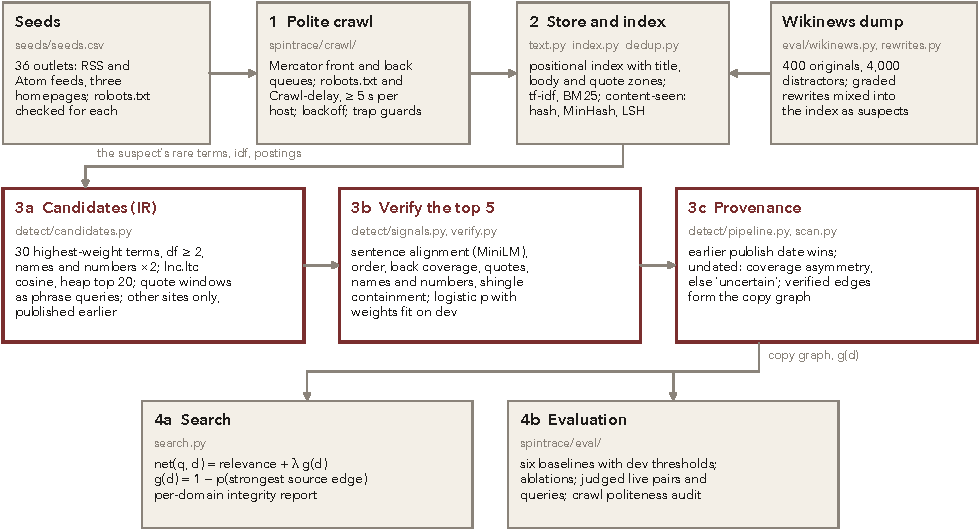
\includegraphics[width=0.94\textwidth]{figures/pipeline.pdf}
  \caption{The SpinTrace pipeline. Oxblood boxes are the detection stage that extends the content-seen check; paths are under \code{spintrace/}.}
  \label{fig:pipeline}
\end{figure}

\begin{table}[t]
  \centering\small
  \caption{IR concepts in SpinTrace, grouped by the five lecture topics listed in the assignment. Code paths are under \code{spintrace/}. Outside the syllabus, BM25 and dense retrieval serve as baselines (\code{index.py}, \code{eval/run.py}).}
  \label{tab:concepts}
  \footnotesize
  \begin{tabularx}{\textwidth}{@{}P{2.5cm}P{5.4cm}LP{3.2cm}@{}}
    \toprule
    \hrow \hd{Lecture topic} & \hd{Concepts we use} & \hd{Why SpinTrace needs them} & \hd{Code} \\
    \midrule
    {\headfont Boolean retrieval} & Inverted index (dictionary and postings); postings intersection in increasing df order & Phrase queries and the candidate query both walk postings lists & \code{index.py} \\
    \addlinespace[2pt]
    {\headfont Term vocabulary and postings} & Tokenisation, case and accent folding, numbers as values; Porter stemming, compared with none; positional index and phrase queries; precision and recall & One pipeline for index, shingles and queries; quotes survive rewriting, so they become phrase queries & \code{text.py}\newline\code{index.py}\newline\code{eval/report.py} \\
    \addlinespace[2pt]
    {\headfont tf-idf and the vector space model} & Jaccard over shingles; idf; lnc.ltc tf-idf; cosine with length normalisation & Jaccard is the check we extend; rare terms carry the evidence; summaries are short, so length normalisation matters & \code{dedup.py}\newline\code{index.py} \\
    \addlinespace[2pt]
    {\headfont Scoring and result assembly} & Index elimination (high-idf terms) with heap top-K; title, body and quote zones; parametric filter on publish date; static quality g(d) and net score & Query only the terms a rewrite keeps; a source must be published first; originals should rank above their copies & \code{detect/candidates.py}\newline\code{detect/scan.py}\newline\code{search.py} \\
    \addlinespace[2pt]
    {\headfont Web crawling} & Crawl loop, Mercator front and back queues, politeness, robots.txt; URL normalisation and spider-trap guards; content-seen check (hash, MinHash, LSH); freshness by re-polling feeds & Collect news without burdening sites; the content-seen check is what SpinTrace extends & \code{crawl/}\newline\code{dedup.py} \\
    \bottomrule
  \end{tabularx}
\end{table}

\paragraph{Crawl} \code{crawl/frontier.py} follows Mercator's split between front queues for priority and back queues for politeness~\cite{heydon1999}. Each host keeps three priority levels (feed and sitemap entries, article-shaped links, everything else) drawn with bias 8:3:1, and a heap of next-allowed fetch times picks the host. Priority sits in one function, \code{priority()}, so a farm-aware policy can replace it later. \code{crawl/robots.py} fetches and stores robots.txt per host and obeys Crawl-delay. The delay is max(Crawl-delay,~5\,s), enforced by the heap and again by a guard before every request. A 5xx, a 429 or a refusal (401, 403, 405, 451) doubles the delay, Retry-After is honoured, and a host is dropped after 5 consecutive errors. Redirects are not followed automatically, so a redirect target goes back through robots.txt and the delay. \code{crawl/urlnorm.py} lowercases the host, drops fragments and tracking parameters and sorts the query. Trap guards reject long, deep, repetitive or parameter-heavy URLs and cap a host at 1,500 pages. A document is trafilatura's main text of at least 120 words plus a publish date from page metadata or the feed. The date matters later, for provenance.

\paragraph{Text and index} \code{text.py} is the one normalisation pipeline for the index, the shingles and the queries: NFKC, case and accent folding, and numbers kept as values so that ``1,394'' matches ``1394''. Stopwords stay in the postings because phrase queries need every position. \code{index.py} builds a positional index with three zones (title, body, quote) and computes lnc.ltc tf-idf and BM25 (\textit{k}\textsubscript{1}~=~1.2, \textit{b}~=~0.75). Phrase queries intersect postings in increasing df order.

\paragraph{Content-seen check} \code{dedup.py} is the textbook check that SpinTrace extends: an exact hash of the normalised text, word 5-gram shingles, MinHash with 128 permutations (estimate error about 0.09) and LSH with 32 bands of 4 rows, whose knee at Jaccard 0.42 catches light edits~\cite{broder1997,iir2008}. It stays in the crawler and runs first. It is also the baseline we have to beat.

\paragraph{Rare-term candidate query} \code{detect/candidates.py} turns a suspect into a query of its 30 highest-weight body terms with df~≥~2, boosting names and numbers by 2. This is index elimination in the textbook sense~\cite[ch.~7]{iir2008}: only the postings of high-idf terms are walked, scores accumulate term at a time, and a heap returns the top 20. Terms with df~=~1 are left out because they can only match the suspect itself. We score with lnc.ltc because it puts idf on the query side only, so the rare terms decide, and cosine length normalisation keeps long articles from winning, which matters when the suspect is a short summary. Quotes are cut into 6-token windows (step 3) and run as phrase queries on the positional index; a rewrite may trim a quote, and any intact window is evidence. A parametric filter keeps only documents from other sites published before the suspect.

\paragraph{Verification} \code{detect/signals.py} and \code{detect/verify.py} check the top 5 candidates. Each signal is an independent scorer: sentence alignment coverage (two sentences match at MiniLM cosine ≥~0.62), the mean alignment score, whether aligned sentences keep their order, back coverage of the candidate, word overlap inside aligned pairs, quote overlap, overlap of names and numbers, shingle containment and the rare-term cosine from retrieval. A class-balanced logistic regression fit on dev pairs combines them, with the threshold that maximises dev F1.

\paragraph{Provenance, g(d) and net score} \code{detect/pipeline.py} orders each verified pair by publish date. If a date is missing it uses coverage asymmetry (the side covered by the other, with margin 0.2), because a summary covers less of its source than the source covers of it; failing that it answers ``uncertain''. \code{detect/scan.py} turns verified edges into a copy graph and sets the static quality to g(d) = 1 − p(strongest source edge), so originals keep g~=~1 and confirmed copies fall towards 0. \code{search.py} ranks by \textit{net}(q,\,d)~=~\textit{relevance}(q,\,d)~+~λ\,g(d) over weighted title and body zones. We chose λ on dev queries from \{0, 0.1, \ldots, 0.8\}; the tuned value is 0.1, small enough that relevance dominates and g(d) mostly breaks ties between an original and its copies.

\section{Beyond IR}

\paragraph{Sentence embeddings} all-MiniLM-L6-v2 (sentence-transformers~\cite{reimers2019}) maps sentences to vectors so that a paraphrased sentence lands near its source. In the detection path it does one job: aligning sentences between a suspect and the five candidates IR returned. The ablations (Appendix, Table~\ref{tab:ablations}) show how the two halves depend on each other. Keeping only the IR signals drops macro F1 over the six levels from 0.896 to 0.802 and raises the false-positive rate on facts-only articles from 0.156 to 0.444. Dropping verification and trusting retrieval alone gives 0.595. In the other direction, swapping the IR candidates for dense-retrieval candidates gives 0.894, so on this corpus the IR stage is not more accurate than dense retrieval as a candidate generator. What it adds is evidence a person can read (which rare terms and quotes matched) and a higher share of sources ranked first: 0.993 against 0.961 for dense retrieval, which ranks the true source first for only 0.83 of SEO rewrites and summaries. A scikit-learn logistic regression combines the ten signals; we chose it for its few parameters and readable weights (\code{results/verifier.json}).

\paragraph{LLM-generated test data} Meta Llama 3.2 3B, run locally through Ollama, wrote the SEO-friendly rewrites, the summaries, the English--German--English round trips and the facts-only articles. They are evaluation data only.

\paragraph{Libraries, in IR terms} \code{requests} is the fetcher; \code{trafilatura} does boilerplate removal, deciding what the document is; \code{lxml} parses links, RSS, Atom and sitemaps; \code{urllib.robotparser} parses robots.txt rules, while fetching, caching and delay policy are ours; \code{nltk} supplies the Porter stemmer and WordNet (used only to make synonym-spun test rewrites); \code{mwparserfromhell} strips wikitext from the Wikinews dump; \code{warcio} reads the CC-NEWS file. Every IR component in Table~\ref{tab:concepts}, BM25 included, is our own code.

\section{Novelty and creativity}

\begin{table}[h]
  \centering\small
  \caption{Tools in use today and why they miss AI rewrites: each either matches surface text or never names a source.}
  \label{tab:existing}
  \footnotesize\begin{tabularx}{\textwidth}{@{}P{4.9cm}P{4.6cm}L@{}}
    \toprule
    \hrow \hd{Approach} & \hd{Catches} & \hd{Why it fails on AI rewrites} \\
    \midrule
    Exact hashing (content-seen) & identical copies & any edit breaks the hash \\
    Shingles with MinHash or SimHash & near-copies, light edits & paraphrases share few shingles \\
    Plagiarism checkers & verbatim reuse & missed 79\% of sources in NewsGuard's test \\
    Domain blocklists & known farm domains & manual and stale; new domains slip through \\
    AI-text detectors & text that looks machine-written & unreliable, and never name the source \\
    \ours SpinTrace & rewrites at any intensity, with their original & weak spots measured in Section~\ref{sec:eval} \\
    \bottomrule
  \end{tabularx}
\end{table}

Beyond the tools in Table~\ref{tab:existing}, the obvious baseline for this track is a shingle near-duplicate detector over a crawl. SpinTrace differs from it in four places. Candidate sources come from the facts a rewrite keeps, as an index-elimination query over the crawler's own inverted index, instead of from surface overlap or from embedding everything and ranking by cosine. A verdict has a direction: the earlier article is the source, or, without dates, the one that covers the other. The verdicts feed back into ranking through g(d), so detection changes what users see. And we test it where the baseline breaks (graded rewrite intensities) and where a paraphrase detector is most likely to be wrong: independent articles about the same event, which share names and numbers without being copies. Every component is textbook IR; what is new is putting them together at the crawler's content-seen step and measuring where the result fails. A GitHub API search in October 2026 found blocklists and generic plagiarism checkers, but no project combining a crawler, paraphrase-aware detection and provenance tracing.

\section{Evaluation}
\label{sec:eval}

\paragraph{Setup} Positives are rewrites of 400 Wikinews originals at six intensities: exact copy, light edit, WordNet synonym spin, an LLM ``SEO-friendly'' rewrite like the one NewsGuard tested, an LLM summary, and an LLM round trip through German. Negatives are the originals themselves, crawl hard negatives (same event, another outlet, published within 3 days, at least 3 shared rare names, and no shingle containment above 0.1 against any earlier document; median gap 10.5\,h, 77\% within 24\,h), and facts-only articles that the LLM wrote from an original's topic, names, numbers and quotes without seeing its text. Every item is scored against the full index of 20,860 documents (the crawl, the originals, 4,000 Wikinews distractors and all rewrites), except that a rewrite cannot see other rewrites of its own original. We split by original story, so a story and all its rewrites fall on one side. The verifier and every method's threshold are fit on the dev split; every number below is from the test split (190 items each for exact, light and synonym, 90 SEO, 90 summary, 45 translation; 190 originals, 301 hard negatives and 90 facts-only as negatives). The baselines are exact hash, MinHash Jaccard over LSH candidates, shingle containment against every earlier document (the best case for shingles), full-document tf-idf cosine, full-document BM25 normalised by the suspect's self-score, and dense cosine of mean MiniLM sentence vectors. Each gets its best dev threshold.

\subsection{Detecting derived articles}

\begin{table}[t]
  \centering\small
  \caption{Test F1 per rewrite level (negatives pooled) and false-positive rate on same-event negatives. Thresholds tuned on dev.}
  \label{tab:f1}
  \setlength{\tabcolsep}{4pt}
  \begin{tabularx}{\textwidth}{@{}l*{8}{R}@{}}
    \toprule
    \hrow \hd{Method} & \hd{exact} & \hd{light} & \hd{synonym} & \hd{seo} & \hd{summary} & \hd{transl.} & \hdd{FPR}{hard neg} & \hdd{FPR}{facts-only} \\
    \midrule
    \ours SpinTrace & 0.960 & 0.960 & 0.960 & 0.782 & 0.902 & 0.816 & 0.007 & 0.156 \\
    Exact hash & 0.995 & 0.000 & 0.000 & 0.000 & 0.000 & 0.000 & 0.000 & 0.022 \\
    MinHash Jaccard & 0.992 & 0.990 & 0.322 & 0.021 & 0.000 & 0.000 & 0.000 & 0.033 \\
    Shingle containment & 0.850 & 0.850 & 0.850 & 0.573 & 0.681 & 0.555 & 0.090 & 0.433 \\
    tf-idf cosine & 0.922 & 0.922 & 0.920 & 0.723 & 0.659 & 0.695 & 0.063 & 0.144 \\
    BM25 & 0.927 & 0.927 & 0.922 & 0.636 & 0.852 & 0.740 & 0.043 & 0.189 \\
    Dense cosine & 0.671 & 0.671 & 0.671 & 0.436 & 0.332 & 0.314 & 0.502 & 0.311 \\
    \bottomrule
  \end{tabularx}
\end{table}

\begin{figure}[t]
  \centering
  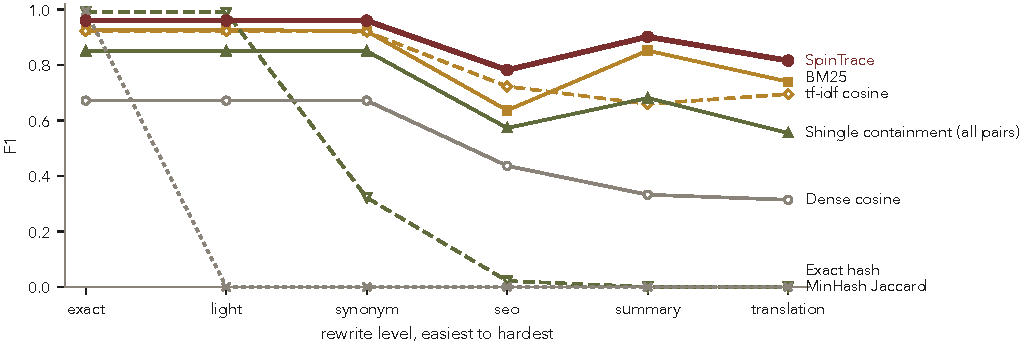
\includegraphics[width=0.98\textwidth]{figures/detection_f1_by_level.pdf}
  \caption{Detection F1 by rewrite intensity (test split). Shingle-based checks are near perfect while the words stay the same and collapse once they change.}
  \label{fig:f1}
\end{figure}

Table~\ref{tab:f1} and Figure~\ref{fig:f1} are the headline result. MinHash Jaccard goes from 0.990 on light edits to 0.322 on synonym spins and 0.021 on SEO rewrites; exact hash scores 0 after any edit. SpinTrace holds 0.960 through the synonym level and ends at 0.782 on SEO rewrites, 0.902 on summaries and 0.816 on round-trip translations, the best F1 at every level after light edits. On SEO rewrites its precision is 0.809 and its recall 0.756.

It loses at the easy end. Exact hash (0.995) and MinHash (0.992 and 0.990) beat its 0.960 on exact copies and light edits, and they cost almost nothing. SpinTrace's threshold is tuned for paraphrases, and the same-story negatives it still flags cost it precision (0.922) at every level. In a crawler the two should run together: the textbook check first, SpinTrace for what it lets through. BM25 comes within 0.05 on summaries (0.852), and full-document tf-idf flags slightly fewer facts-only articles (14.4\% against 15.6\%) while missing far more rewrites. On crawl hard negatives SpinTrace's false-positive rate is 0.007, while dense cosine flags half of them (0.502): to an embedding of the whole article, the same story looks like a copy.

\subsection{Ranking the original first}

SpinTrace ranks the true source first for 0.998 of test positives (MRR 0.998, Recall@20 1.000), and most baselines come close: full-document BM25 reaches 0.996, tf-idf cosine 0.993, shingle containment 0.987 and dense cosine 0.961. MinHash (0.526) and exact hash (0.239) only rank sources they can detect at all. Ranking the right source is easy for sparse methods on this corpus; the case for the rare-term query is in its cost.

\subsection{Index elimination and cost}

\begin{figure}[t]
  \begin{minipage}[t]{0.44\textwidth}
    \vspace{0pt}
    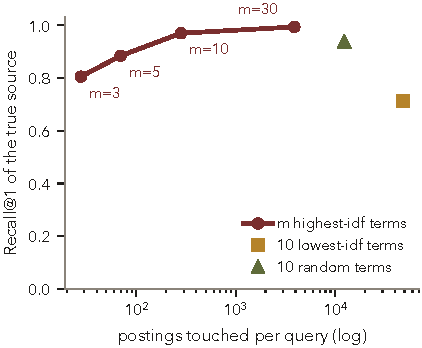
\includegraphics[width=\textwidth]{figures/index_elimination.pdf}
    \captionof{figure}{Recall@1 of the true source from the m highest-idf terms, against postings touched (test positives).}
    \label{fig:elim}
  \end{minipage}\hfill
  \begin{minipage}[t]{0.53\textwidth}
    \vspace{6pt}
    \small\setlength{\tabcolsep}{4pt}
    \captionof{table}{Cost per suspect, averaged over test items.}
    \label{tab:cost}
    \begin{tabularx}{\textwidth}{@{}lRRR@{}}
      \toprule
      \hrow \hd{Method} & \hd{ms} & \hdd{docs}{compared} & \hdd{postings}{touched} \\
      \midrule
      \ours SpinTrace & 23.2 & 20 & 8,293 \\
      Full-document query & -- & -- & 745,985 \\
      Shingle containment & 58.9 & 8,165 & -- \\
      tf-idf cosine & 12.0 & 8,165 & -- \\
      BM25 & 10.8 & 8,165 & -- \\
      Dense cosine & 1.4 & 8,165 & -- \\
      MinHash Jaccard & 0.1 & -- & -- \\
      Exact hash & 0.0 & -- & -- \\
      \bottomrule
    \end{tabularx}
  \end{minipage}
\end{figure}

Figure~\ref{fig:elim} varies the number m of rare terms in the query. Three terms find the source at rank 1 for 0.805 of positives while touching 28 postings; ten terms reach 0.970 with 282 postings; our setting of 30 reaches 0.994 with 3,891. Ten random terms reach 0.937 but touch 12,365 postings, and the ten most common terms reach only 0.713 with 48,375. The rarest terms are both the cheapest query and the most accurate one, which is the premise of Section~2 in one chart.

Table~\ref{tab:cost} gives cost per suspect. SpinTrace touches 8,293 postings, about 1\% of the 745,985 a full-document query touches, and only 20 documents reach the expensive comparison; all-pairs shingle containment compares every earlier document (8,165 on average) and takes 58.9\,ms. SpinTrace is not the fastest in wall-clock time, though: the baselines that compare precomputed vectors take 1.4 to 12.0\,ms against its 23.2\,ms.

\subsection{Originals and copies in search}

\begin{table}[t]
  \centering\small
  \caption{Search with and without g(d) (λ~=~0.1, tuned on dev). Synthetic: test queries from Wikinews titles, body-only relevance. Live: our 15 judged queries over the crawl, under each way of combining the two judges.}
  \label{tab:search}
  \begin{tabularx}{\textwidth}{@{}ll*{4}{R}@{}}
    \toprule
    \hrow \hd{Queries} & \hd{Setting} & \hd{P@10} & \hd{nDCG@10} & \hdd{original}{first} & \hdd{originals in}{relevant top 10} \\
    \midrule
    Synthetic & relevance only & 0.533 & 0.837 & 0.100 & 0.195 \\
    \ours & with g(d) & 0.524 & 0.886 & 0.526 & 0.203 \\
    \addlinespace[2pt]
    Live, either judge & relevance only & 0.933 & 0.973 & 0.867 & 0.927 \\
    \ours & with g(d) & 0.933 & 0.973 & 0.867 & 0.953 \\
    \addlinespace[2pt]
    Live, both judges & relevance only & 0.573 & 0.811 & 0.600 & 0.924 \\
    \ours & with g(d) & 0.560 & 0.803 & 0.600 & 0.963 \\
    \bottomrule
  \end{tabularx}
\end{table}

On synthetic queries, where we know which document is the original, g(d) puts the original first for 52.6\% of queries instead of 10\%, and nDCG@10 rises from 0.837 to 0.886; P@10 dips from 0.533 to 0.524 (Table~\ref{tab:search}). Our 15 judged live queries do not separate the rankings. When either judge's ``relevant'' counts, 93.5\% of judged results were relevant, so P@10 (0.933) and nDCG@10 (0.973) are identical with and without g(d), and the only change is the share of originals among the relevant top 10, from 0.927 to 0.953. When both judges must agree, nDCG@10 is slightly lower with g(d) (0.803 against 0.811).

\subsection{Human judgments of live flags}

Both of us labelled all 174 pairs that SpinTrace flagged in the live crawl. We judged blind: the judging page hides SpinTrace's score and verdict and the other judge's label. Live precision depends on how the two labels are combined: 0.845 if either judge says derived (our convention, and the lenient one), 0.437 if both must, and 0.738 on the 103 pairs we agreed on. We agreed on only 59\% of pairs (Cohen's kappa 0.123); Judge~1 called 103 derived and Judge~2 called 120. On search results agreement was 0.636 (kappa 0.161) over 154 judged results. Judge~1's not-derived pairs have much less exact overlap (median shingle containment 0.38, against 0.85 for derived pairs), which fits the sentence alignment matching independent coverage of one event.

\subsection{Documented farm pairs}

Two of four NewsGuard-documented pairs loaded from the Wayback Machine; for the other two the report does not name the originals. The New York Times original of a GlobalVillageSpace rewrite is retrieved first among 20,860 documents, verified at p~=~0.999 and traced. The Wired original of a TopGolf.kr page is also retrieved first but not verified (p~=~0.0): that page is AI title suggestions plus a reshaped deals list, and our verifier was trained on prose. Two pairs are anecdotes, not a measurement.

\subsection{Crawler correctness and politeness}

\begin{table}[t]
  \centering\small
  \caption{Crawl statistics from \code{crawl-report}. Every fetched URL is re-checked against the stored robots.txt.}
  \label{tab:crawl}
  \begin{tabularx}{\textwidth}{@{}Xr@{\hspace{2.2em}}Xr@{}}
    \toprule
    \hrow \hd{Measure} & \hd{Value} & \hd{Measure} & \hd{Value} \\
    \midrule
    Crawl time (hours), one process & 13.49 & Disallowed URLs fetched & 0 \\
    Page requests & 43,683 & Fetches audited against robots.txt & 43,674 \\
    robots.txt requests & 620 & URLs skipped by robots.txt & 512 \\
    Documents saved & 32,513 & Smallest gap to one host (s) & 0.29 \\
    Pages per minute & 54.0 & Requests under the 5\,s floor & 9 \\
    Hosts & 118 & Backoffs & 77 \\
    Median freshness (min, 968 articles) & 69.7 & Trap guards fired & 2,569 \\
    Exact / near duplicates & 792 / 1,099 & Duplicate rate & 0.0695 \\
    \bottomrule
  \end{tabularx}
\end{table}

Table~\ref{tab:crawl} summarises the crawl. No disallowed URL was fetched among 43,674 audited fetches, and 512 URLs were skipped because robots.txt disallowed them. The delay floor was not perfect: 9 requests came less than 5\,s after the previous one to the same host, the closest 0.29\,s apart. The last of them was at 23:45 on 6 October; the crawl report had exposed a race in the politeness check, which we fixed at 23:46.

\section{Limitations and next steps}

The boundary between ``same story'' and ``copied'' is where SpinTrace is weakest. Articles written from an original's facts and quotes alone are still flagged 15.6\% of the time, and recall on SEO rewrites is 0.76 at the dev-tuned threshold. The LLM rewrites closest to the ones NewsGuard tested are where SpinTrace misses most.

The live results say less about farms than we hoped. The crawl contained no actual farm sites; our seeds turned up aggregators and outlets that republish agency copy, and the live flags are mostly wire syndication (PTI, ANI, Reuters). When two outlets print the same agency story, SpinTrace credits whichever outlet we crawled first, because the agency itself is not crawled. Our only real farm cases are the two NewsGuard pairs.

Quote phrase matching, which we expected to be a key signal, turned out neutral. Retrieval with quote phrases finds the source first for 0.993 of positives against 0.994 without them, and removing quote overlap from the verifier leaves macro F1 at 0.896. Copies and independent coverage share quotes alike, since outlets quote the same speaker. The evidence is in names and numbers: removing their overlap drops macro F1 to 0.884 and raises the facts-only false-positive rate to 0.222. Our mined hard negatives share no text, so same-event pairs that share quotes are not yet tested.

Judge agreement was low (kappa 0.123 on live flags, 0.161 on search), so live precision is a range from 0.437 to 0.845, not a number. The synthetic test rewrites come from one 3B model; stronger models paraphrase more and would be harder. Publish dates are trusted, so a farm that backdates its pages escapes the earlier-only filter. Dropping the filter costs little in retrieval (Recall@1 0.989 against 0.993), but undated provenance mostly abstains on same-length rewrites and works mainly for summaries (Appendix, Table~\ref{tab:undated}). Scale is modest: one crawler process and 32.5k articles over 13.5 hours, of which the evaluation used about the first 16k.

\paragraph{Course-project roadmap} We plan to continue SpinTrace as our course project, in this order:
\begin{enumerate}
  \item Farm-aware focused crawling: raise the priority of domains with high derivative rates through the \code{priority()} hook.
  \item Recognise agency datelines and bylines, so syndicated copies point to the agency rather than to the first outlet crawled.
  \item A harder evaluation: rewrites from stronger LLMs, same-event negatives that share quotes, and an external benchmark (PAN~\cite{potthast2010} or METER).
  \item Signal weights learned from judged live pairs, after a second labelling round with a tighter guide.
  \item Adaptive recrawl scheduling, more fetcher threads and a larger CC-NEWS index; later, English-to-Hindi derivatives.
\end{enumerate}

\section{Work division and AI-use declaration}

\paragraph{Work division} Both of us wrote the plan, chose the track and the claim, and judged the live flags and search results independently. The commit history follows this split.

{\footnotesize
  \setlength{\tabcolsep}{0.9em}
  \begin{tabularx}{\textwidth}{@{}LL@{}}
    \toprule
    \hrow \hd{Nishita Kadali} & \hd{Pustak Pathak} \\
    \addlinespace[4pt]
    \textit{Crawler, IR core and detection signals} & \textit{Pipeline groundwork and evaluation} \\
    \midrule
    \begin{wdlist}
      \item Polite crawl loop, trap guards, frontier hardening
      \item Positional zoned index, tf-idf, BM25, MinHash, LSH
      \item Detection signals and the copy-graph scan
      \item Originality-aware search; inspect and trace commands
      \item Storage, export, re-crawl and run-all scripts; README
    \end{wdlist}
    &
    \begin{wdlist}
      \item URL normalisation, robots cache, frontier, extraction
      \item Candidate retrieval, verification and provenance stages
      \item Wikinews rewrites, hard negatives, NewsGuard pairs
      \item Baselines, ablations, scale run, charts, judge agreement
      \item Unit tests, critique notes, judging tool, demo web app
    \end{wdlist}
    \\
    \bottomrule
  \end{tabularx}
\par}

\paragraph{AI-use declaration}
\begin{itemize}[itemsep=0.25em]
  \item We used Claude Code (Anthropic, Claude Opus 5.5) as a coding agent throughout the build.
  \item From our plan and brief (\code{PLAN.md}, \code{CLAUDE.md}) it generated the package code under \code{spintrace/}, the tests, the command-line interface, the evaluation code and charts, the README, \code{PROGRESS.md} and the critique notes in \code{notes/}.
  \item We wrote the plan, the brief and the seed strategy, and reviewed the code and the results.
  \item Meta Llama 3.2 3B, run locally through Ollama, generated the synthetic SEO rewrites, summaries, round-trip translations and facts-only articles, which are evaluation data only.
  \item The pretrained all-MiniLM-L6-v2 model serves verification and the dense baseline.
  \item No AI system labelled evaluation data: synthetic labels come from how the rewrites were built, hard negatives from a rule-based miner, and live labels from the two of us.
\end{itemize}

\clearpage
\renewcommand{\refname}{References}
\begin{thebibliography}{9}
\small
\setlength{\itemsep}{0.2em}

\bibitem{ng2023} J.~Brewster, M.~Wang and C.~Palmer. Plagiarism-Bot? How low-quality websites are using AI to deceptively rewrite content from mainstream news outlets. \textit{NewsGuard Misinformation Monitor}, 24 August 2023. \url{https://www.newsguardtech.com/misinformation-monitor/august-2023}

\bibitem{ng2026} M.~Sadeghi et al. Tracking AI-enabled misinformation: AI content farm sites and top false claims generated by artificial intelligence tools. \textit{NewsGuard AI Tracking Center}, updated 23 June 2026, accessed 7 October 2026. \url{https://www.newsguardtech.com/special-reports/ai-tracking-center}

\bibitem{broder1997} A.~Z.~Broder. On the resemblance and containment of documents. In \textit{Proceedings of Compression and Complexity of Sequences (SEQUENCES '97)}, pages 21--29. IEEE, 1997.

\bibitem{manku2007} G.~S.~Manku, A.~Jain and A.~Das~Sarma. Detecting near-duplicates for web crawling. In \textit{Proceedings of the 16th International Conference on World Wide Web (WWW '07)}, pages 141--150. ACM, 2007.

\bibitem{heydon1999} A.~Heydon and M.~Najork. Mercator: A scalable, extensible web crawler. \textit{World Wide Web}, 2(4):219--229, 1999.

\bibitem{iir2008} C.~D.~Manning, P.~Raghavan and H.~Sch\"utze. \textit{Introduction to Information Retrieval}. Cambridge University Press, 2008.

\bibitem{robertson2009} S.~Robertson and H.~Zaragoza. The probabilistic relevance framework: BM25 and beyond. \textit{Foundations and Trends in Information Retrieval}, 3(4):333--389, 2009.

\bibitem{reimers2019} N.~Reimers and I.~Gurevych. Sentence-BERT: Sentence embeddings using Siamese BERT-networks. In \textit{Proceedings of EMNLP-IJCNLP 2019}, pages 3982--3992. ACL, 2019.

\bibitem{potthast2010} M.~Potthast, B.~Stein, A.~Barr\'on-Cede\~no and P.~Rosso. An evaluation framework for plagiarism detection. In \textit{Coling 2010: Posters}, pages 997--1005, 2010.

\end{thebibliography}

{\small
\textit{Data credits.} English Wikinews (CC BY 2.5, Wikinews contributors), read from the official Wikimedia dump; the live crawl from 36 seed outlets, of which only URLs and features are committed; NewsGuard-documented farm pages and their originals via the Internet Archive Wayback Machine; one Common Crawl CC-NEWS file (6 October 2026) for the scale experiment only; all-MiniLM-L6-v2 (Apache 2.0).\par}

\clearpage
\appendix
\renewcommand{\thetable}{A\arabic{table}}
\renewcommand{\thefigure}{A\arabic{figure}}
\setcounter{table}{0}
\setcounter{figure}{0}
\section*{Appendix}
\addcontentsline{toc}{section}{Appendix}

All numbers are on the test split, with anything tuned fit on dev.

\begin{table}[H]
  \centering\small
  \caption{SpinTrace precision, recall and share of positives traced to the correct source, per level.}
  \label{tab:pr}
  \begin{tabularx}{0.75\textwidth}{@{}l*{4}{R}@{}}
    \toprule
    \hrow \hd{Level} & \hd{Precision} & \hd{Recall} & \hd{F1} & \hd{Source correct} \\
    \midrule
    exact & 0.922 & 1.000 & 0.960 & 0.995 \\
    light & 0.922 & 1.000 & 0.960 & 0.995 \\
    synonym & 0.922 & 1.000 & 0.960 & 1.000 \\
    seo & 0.809 & 0.756 & 0.782 & 0.756 \\
    summary & 0.845 & 0.967 & 0.902 & 0.967 \\
    translation & 0.724 & 0.933 & 0.816 & 0.933 \\
    \bottomrule
  \end{tabularx}
\end{table}

\begin{table}[H]
  \centering\small
  \caption{Ablations: test macro F1 over the six levels, with the verifier refit on dev without the signal.}
  \label{tab:ablations}
  \begin{tabularx}{0.85\textwidth}{@{}l*{3}{R}@{}}
    \toprule
    \hrow \hd{Variant} & \hd{Macro F1} & \hd{FPR hard neg} & \hd{FPR facts-only} \\
    \midrule
    \ours Full & 0.896 & 0.007 & 0.156 \\
    minus rare-term cosine & 0.882 & 0.010 & 0.211 \\
    minus shingle containment & 0.892 & 0.007 & 0.167 \\
    minus alignment coverage & 0.884 & 0.007 & 0.211 \\
    minus alignment mean & 0.896 & 0.010 & 0.144 \\
    minus alignment order & 0.885 & 0.010 & 0.178 \\
    minus back coverage & 0.887 & 0.007 & 0.189 \\
    minus ordered coverage & 0.885 & 0.010 & 0.178 \\
    minus aligned word overlap & 0.900 & 0.007 & 0.144 \\
    minus quote overlap & 0.896 & 0.007 & 0.156 \\
    minus names and numbers overlap & 0.884 & 0.007 & 0.222 \\
    No embedding signals (IR signals only) & 0.802 & 0.007 & 0.444 \\
    Dense candidates instead of IR & 0.894 & 0.007 & 0.156 \\
    IR retrieval only, no verification & 0.595 & 0.242 & 0.767 \\
    \bottomrule
  \end{tabularx}
\end{table}

Removing aligned word overlap raises macro F1 slightly on test (0.900 against 0.896). It was added in our third critique round after cross-validation on dev only, and we kept it rather than tune on test.

\begin{table}[H]
  \centering\small
  \caption{Retrieval variants: share of test positives whose true source is ranked first and in the top 20.}
  \label{tab:variants}
  \begin{tabularx}{0.75\textwidth}{@{}l*{2}{R}@{}}
    \toprule
    \hrow \hd{Variant} & \hd{Recall@1} & \hd{Recall@20} \\
    \midrule
    \ours Rare terms + quote phrases & 0.993 & 1.000 \\
    Rare terms only (no quotes) & 0.994 & 1.000 \\
    No fact boost & 0.991 & 0.999 \\
    No date filter (dates untrusted) & 0.989 & 1.000 \\
    Rare terms, Porter stemming & 0.996 & 1.000 \\
    Dense retrieval & 0.961 & 1.000 \\
    Full-document tf-idf & 0.993 & 1.000 \\
    \bottomrule
  \end{tabularx}
\end{table}

With Porter stemming the rare-term query ranks the true source first for 0.996 of positives, against 0.993 for our unstemmed query with quote phrases, so stemming helps only at the margin.

\begin{table}[H]
  \centering\small
  \caption{Provenance without dates: coverage asymmetry on the known pair, margin 0.2.}
  \label{tab:undated}
  \begin{tabularx}{0.85\textwidth}{@{}l*{4}{R}@{}}
    \toprule
    \hrow \hd{Level} & \hd{n} & \hd{Suspect called derived} & \hd{Direction reversed} & \hd{Uncertain} \\
    \midrule
    exact & 190 & 0.000 & 0.000 & 1.000 \\
    light & 190 & 0.079 & 0.000 & 0.921 \\
    synonym & 190 & 0.000 & 0.000 & 1.000 \\
    seo & 90 & 0.167 & 0.033 & 0.800 \\
    summary & 90 & 0.956 & 0.000 & 0.044 \\
    translation & 45 & 0.178 & 0.022 & 0.800 \\
    hard negative & 301 & 0.053 & 0.030 & 0.917 \\
    facts-only & 90 & 0.267 & 0.000 & 0.733 \\
    \bottomrule
  \end{tabularx}
\end{table}

\begin{table}[H]
  \centering\small
  \caption{Scale: the same test items with the index grown to 24,501 documents by 3,637 CC-NEWS articles from the same days. Verifier and threshold not refit. False-positive rates at this size: originals 0.000, hard negatives 0.007, facts-only 0.156.}
  \label{tab:scale}
  \begin{tabularx}{\textwidth}{@{}l*{6}{R}@{}}
    \toprule
    \hrow \hd{Level} & \hd{Recall@1} & \hd{Recall@20} & \hd{Full-doc tf-idf Recall@1} & \hd{F1} & \hd{Postings touched} & \hd{Postings, full-doc query} \\
    \midrule
    exact & 1.000 & 1.000 & 1.000 & 0.960 & 9,698 & 811,153 \\
    light & 1.000 & 1.000 & 1.000 & 0.960 & 10,694 & 784,633 \\
    synonym & 1.000 & 1.000 & 1.000 & 0.960 & 6,747 & 817,589 \\
    seo & 0.989 & 1.000 & 0.978 & 0.789 & 9,948 & 747,305 \\
    summary & 0.956 & 1.000 & 0.978 & 0.902 & 21,650 & 399,229 \\
    translation & 0.956 & 1.000 & 0.956 & 0.816 & 12,022 & 683,412 \\
    \bottomrule
  \end{tabularx}
\end{table}

\begin{table}[H]
  \centering\small
  \caption{Per-domain integrity in the live crawl: share of a site's articles flagged as derived (top 10 sites).}
  \label{tab:domains}
  \begin{tabularx}{\textwidth}{@{}l*{3}{r}L@{}}
    \toprule
    \hrow \hd{Site} & \hd{Articles} & \hd{Flagged} & \hd{Share} & \hd{Main sources} \\
    \midrule
    devdiscourse.com & 692 & 20 & 0.029 & indiatimes.com (11); independent.co.uk (4); socialnews.xyz (2) \\
    theprint.in & 400 & 11 & 0.028 & indiatimes.com (4); hindustantimes.com (3); devdiscourse.com (1) \\
    independent.co.uk & 608 & 15 & 0.025 & abcnews.com (9); hindustantimes.com (2); france24.com (1) \\
    thehindu.com & 449 & 11 & 0.025 & socialnews.xyz (3); theprint.in (3); abcnews.com (2) \\
    indiatimes.com & 2,324 & 55 & 0.024 & devdiscourse.com (17); hindustantimes.com (13); indianexpress.com (10) \\
    latestly.com & 632 & 11 & 0.017 & dw.com (5); socialnews.xyz (3); abc.net.au (1) \\
    newsx.com & 316 & 5 & 0.016 & devdiscourse.com (4); theprint.in (1) \\
    scroll.in & 585 & 9 & 0.015 & theconversation.com (9) \\
    indianexpress.com & 548 & 8 & 0.015 & hindustantimes.com (2); indiatimes.com (2); devdiscourse.com (1) \\
    cbsnews.com & 339 & 4 & 0.012 & france24.com (3); abcnews.com (1) \\
    \bottomrule
  \end{tabularx}
\end{table}

These shares are flags, not judged derivatives; Section~5.5 gives the judged precision. Many of the source edges are outlets running the same agency story.

\begin{figure}[H]
  \centering
  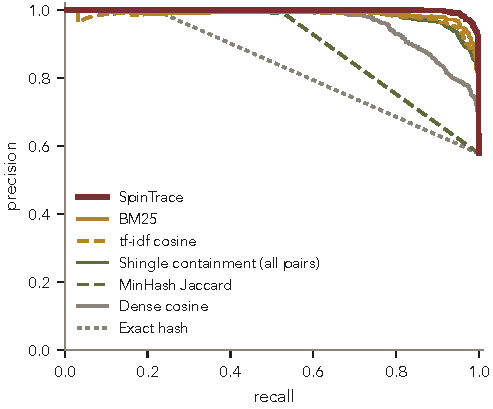
\includegraphics[width=0.55\textwidth]{figures/pr_curve.pdf}
  \caption{Precision and recall over all rewrite levels pooled (test), from each method's score.}
  \label{fig:pr}
\end{figure}

\end{document}
